% =====================================================================
\clearpage
\partieENO{La thermodynamique}

Cette partie traite de la chaleur : à quelle température l'eau du bac va-t-elle se stabiliser, et que faire si elle est trop chaude ? La température de l'eau compte pour les racines : au-dessus d'environ \qty{26}{\celsius}, l'eau contient moins d'oxygène et les maladies des racines progressent. Je commence par le bilan de chaleur du bac (6.1). J'en déduis l'effet de la couleur (6.2), puis la chaleur ajoutée par la pompe (6.3). Je raffine ensuite le bilan avec l'évaporation et le rayonnement (6.4), puis je calcule les pertes par effet Joule de l'installation, à partir des données de l'étude électrique (6.5). Je regarde la chaleur reçue par la tour et les tuyaux (6.6), l'échauffement de l'armoire et de la batterie (6.7), et les solutions si l'eau est trop chaude (6.8). Je termine par ce que je mesurerai (6.9). Il n'y a encore aucune mesure : ce sont des calculs, à partir d'hypothèses signalées.

\Needspace{8\baselineskip}\subsection{Le bilan de chaleur du bac}

\subsubsection*{Ce que je cherche et ce que je suppose}

Je cherche de combien le soleil réchauffe l'eau du bac, et quelle température elle atteint. Le bac reçoit de la chaleur du soleil, en reçoit de la pompe, et en échange avec l'air. Je suppose un bac parallélépipédique de $\qty{0,70}{m} \times \qty{0,45}{m} \times \qty{0,48}{m}$ (volume intérieur proche de \qty{151}{L}, hypothèse à mesurer), un coefficient d'échange avec l'air $h = \qty{8}{W/(m^2\,K)}$ (air calme à peu agité, hypothèse), un éclairement de \qty{800}{W/m^2} sur le dessus à midi, et une irradiation de \qty{4,2}{kWh/m^2/j} (valeur de ma première étude électrique ; la moyenne annuelle de Solargis est de \qty{4,74}{kWh/m^2/j}, partie 5.4). La chaleur massique de l'eau est $c = \qty{4180}{J/(kg\,K)}$ et \qty{152}{L} d'eau pèsent \qty{152}{kg}.

\naturecalc{théorie (formule démontrée, valeurs de fiches techniques et hypothèses ; rien de mesuré)}
\begin{demonstration}[température du bac au cours du temps]
\resultat{\Delta T(t) = \Delta T_{\infty}\left(1 - e^{-t/\tau}\right)}
Je note $T$ la température de l'eau, en °C, $T_a$ celle de l'air, en °C, $\Delta T = T - T_a$ l'élévation, en kelvins, $m$ la masse d'eau, en kg, $c$ sa chaleur massique, en J/(kg$\cdot$K), $C = m\,c$ la capacité thermique, en J/K, $P_s$ la puissance solaire absorbée, en watts, $h$ le coefficient d'échange, en W/(m$^2\cdot$K), $S_t$ la surface totale d'échange du bac, en m$^2$. L'énergie gagnée par l'eau pendant $\mathrm{d}t$ est la puissance reçue moins la puissance perdue vers l'air :
\begin{align*}
C\,\frac{\mathrm{d}T}{\mathrm{d}t} &= P_s - h\,S_t\,(T - T_a)\\
\dimline{\unit{J/K}\times\unit{K/s}=\unit{J/s}=\unit{W}\ ;\ \unit{W/(m^2\,K)}\times\unit{m^2}\times\unit{K}=\unit{W}}
\end{align*}
Comme $T_a$ est constant, $\mathrm{d}T/\mathrm{d}t = \mathrm{d}(\Delta T)/\mathrm{d}t$. Je pose $G_t = h\,S_t$ (en W/K) :
\begin{align*}
C\,\frac{\mathrm{d}(\Delta T)}{\mathrm{d}t} + G_t\,\Delta T &= P_s
\end{align*}
Je divise par $G_t$ et je pose $\tau = C/G_t$ (en secondes) et $\Delta T_{\infty} = P_s/G_t$ :
\begin{align*}
\tau\,\frac{\mathrm{d}(\Delta T)}{\mathrm{d}t} + \Delta T &= \Delta T_{\infty}
\end{align*}
Je sépare les variables : $\dfrac{\mathrm{d}(\Delta T)}{\Delta T_{\infty} - \Delta T} = \dfrac{\mathrm{d}t}{\tau}$. J'intègre de $0$ (où $\Delta T = 0$) à $t$ :
\begin{align*}
-\ln\!\left(\Delta T_{\infty} - \Delta T\right) \Big|_{0}^{t} &= \frac{t}{\tau}\\
\ln\frac{\Delta T_{\infty}}{\Delta T_{\infty} - \Delta T(t)} &= \frac{t}{\tau}\\
\Delta T(t) &= \Delta T_{\infty}\left(1 - e^{-t/\tau}\right)
\end{align*}
L'eau tend donc vers $\Delta T_{\infty}$ avec la constante de temps $\tau$.
\end{demonstration}

\naturecalc{théorie (formule démontrée, valeurs de fiches techniques et hypothèses ; rien de mesuré)}
\begin{demonstration}[capacité thermique, surface et constante de temps]
\resultat{\tau \approx \qty{12,7}{h}}
\begin{align*}
C &= m\,c = \qty{152}{kg} \times \qty{4180}{J/(kg\,K)} \approx \qty{635360}{J/K}\\
\dimline{\unit{kg}\times\unit{J/(kg\,K)}=\unit{J/K}}
\end{align*}
La surface totale d'échange est celle des six faces du bac, deux fois la somme des trois produits de côtés :
\begin{align*}
S_t &= 2\,(L\,l + L\,H_b + l\,H_b)\\
S_t &= 2\,(\qty{0,70}{m}\times\qty{0,45}{m} + \qty{0,70}{m}\times\qty{0,48}{m} + \qty{0,45}{m}\times\qty{0,48}{m})\\
S_t &= 2\,(\qty{0,315}{m^2} + \qty{0,336}{m^2} + \qty{0,216}{m^2})\\
S_t &\approx \qty{1,734}{m^2}\\
\dimline{\unit{m}\times\unit{m}=\unit{m^2}}
\end{align*}
\begin{align*}
G_t &= h\,S_t = \qty{8}{W/(m^2\,K)} \times \qty{1,734}{m^2} \approx \qty{13,87}{W/K}\\
\dimline{\unit{W/(m^2\,K)}\times\unit{m^2}=\unit{W/K}}\\
\tau &= \frac{C}{G_t} = \frac{\qty{635360}{J/K}}{\qty{13,87}{W/K}} \approx \qty{45800}{s} \approx \qty{12,7}{h}\\
\dimline{\dfrac{\unit{J/K}}{\unit{W/K}}=\dfrac{\unit{J}}{\unit{J/s}}=\unit{s}}
\end{align*}
Le bac a une grande inertie : il met environ 13 heures à rattraper 63\,\% de l'écart. Il lisse donc les variations de la journée.
\end{demonstration}

\textbf{Limite sur la surface d'échange.} J'ai compté les six faces du bac comme échangeant avec l'air. Si le fond repose sur un support ou sur le sol, il échange beaucoup moins. Sans le fond (\qty{0,315}{m^2}), la surface vaut $\qty{1,734}{m^2} - \qty{0,315}{m^2} = \qty{1,419}{m^2}$, donc $G_t = \qty{8}{W/(m^2\,K)} \times \qty{1,419}{m^2} \approx \qty{11,35}{W/K}$ et $\tau \approx \qty{15,5}{h}$. Les élévations de température calculées plus bas seraient alors environ 22 \% plus grandes. Mon modèle est donc plutôt prudent sur ce point, et la mesure de $\tau$ du protocole permettra de choisir la bonne surface.

\Needspace{8\baselineskip}\subsection{Pourquoi le bac est peint en blanc}

Une surface absorbe une part $\alpha$ de la lumière du soleil. Pour une surface noire, $\alpha$ est d'environ $0{,}9$ ; pour une surface blanche, environ $0{,}25$ (valeurs usuelles pour les peintures, hypothèses). La puissance absorbée par le dessus du bac, de surface $S_{top} = L\,l = \qty{0,315}{m^2}$ sous $G = \qty{800}{W/m^2}$, vaut $P_s = \alpha\,G\,S_{top}$.

\naturecalc{théorie (formule démontrée, valeurs de fiches techniques et hypothèses ; rien de mesuré)}
\begin{demonstration}[effet de la couleur sur l'élévation de température]
\resultat{\Delta T_{\infty} = \dfrac{\alpha\,G\,S_{top}}{h\,S_t}}
Je reprends $\Delta T_{\infty} = P_s/G_t$ avec $P_s = \alpha\,G\,S_{top}$ et $G_t = \qty{13,87}{W/K}$ :
\begin{align*}
P_{s,noir} &= 0{,}9 \times \qty{800}{W/m^2} \times \qty{0,315}{m^2} = \qty{226,8}{W}\\
P_{s,blanc} &= 0{,}25 \times \qty{800}{W/m^2} \times \qty{0,315}{m^2} = \qty{63,0}{W}\\
\dimline{\unit{W/m^2}\times\unit{m^2}=\unit{W}}
\end{align*}
\begin{align*}
\Delta T_{\infty,noir} &= \frac{\qty{226,8}{W}}{\qty{13,87}{W/K}} \approx \qty{16,3}{K}\\
\Delta T_{\infty,blanc} &= \frac{\qty{63,0}{W}}{\qty{13,87}{W/K}} \approx \qty{4,5}{K}\\
\dimline{\dfrac{\unit{W}}{\unit{W/K}}=\unit{K}}
\end{align*}
Sur les six premières heures de soleil ($t = \qty{21600}{s}$), le facteur $1 - e^{-t/\tau}$ vaut :
\begin{align*}
1 - e^{-21600/45800} &= 1 - e^{-0{,}472} \approx 0{,}376\\
\dimline{\dfrac{\unit{s}}{\unit{s}}=\text{sans unité}}
\end{align*}
\begin{align*}
\Delta T_{noir}(\qty{6}{h}) &= \qty{16,3}{K} \times 0{,}376 \approx \qty{6,1}{K}\\
\Delta T_{blanc}(\qty{6}{h}) &= \qty{4,5}{K} \times 0{,}376 \approx \qty{1,7}{K}\\
\dimline{\text{sans unité}\times\unit{K}=\unit{K}}
\end{align*}
\end{demonstration}

La figure suivante montre comment la température de l'eau du bac monte au cours d'une journée de soleil, selon la couleur du bac.

\begin{figure}[H]
\centering
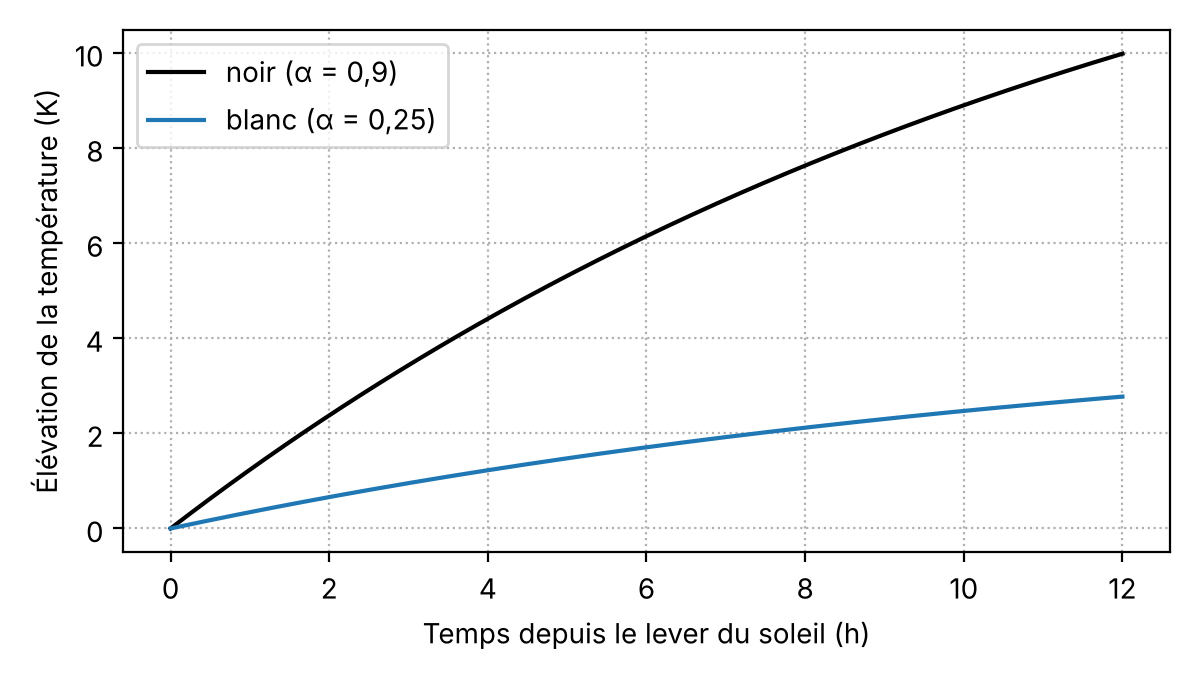
\includegraphics[width=0.72\textwidth]{img/thermo.png}
\caption{Élévation de la température de l'eau du bac au cours d'une journée de soleil, selon la couleur du bac (calcul).}
\end{figure}

Le blanc évite donc environ \qty{4,4}{K} d'échauffement en six heures de plein soleil. Pour la journée entière, avec l'irradiation de \qty{4,2}{kWh/m^2/j} retenue dans ma première étude électrique (soit une puissance moyenne $H/24\,\mathrm{h} = \qty{175}{W/m^2}$), l'élévation moyenne est :

\naturecalc{théorie (formule démontrée, valeurs de fiches techniques et hypothèses ; rien de mesuré)}
\begin{demonstration}[élévation moyenne sur 24 heures]
\resultat{\overline{\Delta T} = \dfrac{\alpha\,H\,S_{top}}{\qty{24}{h}\; h\,S_t}}
La chaleur absorbée sur un jour vaut $\alpha\,H\,S_{top}$ et la chaleur évacuée par kelvin et par jour vaut $24\,h\,G_t$. Analyse dimensionnelle : $\unit{Wh/m^2}\times\unit{m^2}=\unit{Wh}$ et $\unit{h}\times\unit{W/K}=\unit{Wh/K}$. En noir, $0{,}9 \times \qty{4200}{Wh/m^2} \times \qty{0,315}{m^2} = \qty{1190,7}{Wh}$ par jour, et $\qty{24}{h} \times \qty{13,87}{W/K} = \qty{332,9}{Wh/K}$ :
\begin{align*}
\overline{\Delta T}_{noir} &= \frac{\qty{1190,7}{Wh}}{\qty{332,9}{Wh/K}} \approx \qty{3,6}{K}\\
\overline{\Delta T}_{blanc} &= \frac{0{,}25 \times \qty{4200}{Wh} \times 0{,}315}{\qty{332,9}{Wh/K}} = \frac{\qty{330,8}{Wh}}{\qty{332,9}{Wh/K}} \approx \qty{1,0}{K}\\
\dimline{\dfrac{\unit{Wh}}{\unit{Wh/K}}=\unit{K}}
\end{align*}
\end{demonstration}

\Needspace{8\baselineskip}\subsection{La chaleur ajoutée par la pompe}

La pompe est immergée : toute la puissance électrique qui ne sert pas à monter l'eau finit en chaleur dans le bac. La puissance hydraulique est $P_h = \rho\,g\,Q\,H$.

\naturecalc{théorie (formule démontrée, valeurs de fiches techniques et hypothèses ; rien de mesuré)}
\begin{demonstration}[chaleur dégagée par la pompe]
\resultat{\overline{\Delta T}_{pompe} \approx \qty{0,33}{K}}
Je note $\rho = \qty{997}{kg/m^3}$ la masse volumique de l'eau, $g = \qty{9,81}{m/s^2}$, $Q$ le débit en m$^3$/s et $H$ la hauteur manométrique en mètres. La puissance hydraulique est l'énergie potentielle gagnée par seconde par l'eau montée :
\begin{align*}
P_h &= \rho\,g\,Q\,H
\end{align*}
Avec $Q = \qty{388}{L/h} = \qty{1,078e-4}{m^3/s}$ et $H = \qty{2,57}{m} $ (partie 3) :
\begin{align*}
P_h &= \qty{997}{kg/m^3} \times \qty{9,81}{m/s^2} \times \qty{1,078e-4}{m^3/s} \times \qty{2,57}{m}\\
P_h &\approx \qty{2,7}{W}\\
\dimline{\unit{kg/m^3}\times\unit{m/s^2}\times\unit{m^3/s}\times\unit{m}=\unit{kg\,m^2/s^3}=\unit{W}}
\end{align*}
La chaleur dégagée par la pompe en marche est le reste de ses \qty{19}{W} :
\begin{align*}
P_{q} &= \qty{19}{W} - \qty{2,7}{W} = \qty{16,3}{W}\\
\dimline{\unit{W}-\unit{W}=\unit{W}}
\end{align*}
Elle ne marche que \qty{6,75}{h} par jour. La puissance moyenne et l'élévation moyenne de température associée valent :
\begin{align*}
\overline{P}_q &= \qty{16,3}{W} \times \frac{\qty{6,75}{h}}{\qty{24}{h}} \approx \qty{4,6}{W}\\
\overline{\Delta T}_{pompe} &= \frac{\overline{P}_q}{G_t} = \frac{\qty{4,6}{W}}{\qty{13,87}{W/K}} \approx \qty{0,33}{K}\\
\dimline{\unit{W}\times\dfrac{\unit{h}}{\unit{h}}=\unit{W}\ ;\ \dfrac{\unit{W}}{\unit{W/K}}=\unit{K}}
\end{align*}
\end{demonstration}


\textbf{Où va l'énergie hydraulique.} Je retire les \qty{2,7}{W} de puissance hydraulique de la chaleur de la pompe parce qu'ils servent à monter l'eau. Mais l'eau redescend dans le bac par ruissellement et cette énergie est dissipée par les frottements et les turbulences, en grande partie dans l'eau du circuit qui retourne au bac. Le cas le plus défavorable est donc que les \qty{19}{W} entiers chauffent le bac : $\overline{\Delta T}_{pompe} = \qty{19}{W} \times (\qty{6,75}{h}/\qty{24}{h}) / \qty{13,87}{W/K} \approx \qty{0,385}{K}$, soit \qty{0,05}{K} de plus que la valeur retenue. La différence est faible, mais elle va dans le sens d'une eau un peu plus chaude.

\Needspace{8\baselineskip}\subsection{L'évaporation et le rayonnement}

Le bilan du début regroupe tous les échanges avec l'air dans un seul coefficient $h$. Je sépare ici deux effets qui changent la température de l'eau : le rayonnement vers le ciel et l'évaporation. Je vérifie d'abord que la valeur $h = \qty{8}{W/(m^2\,K)}$ est cohérente, puis j'ajoute les deux effets au bilan.

\naturecalc{théorie (formule démontrée, valeurs de fiches techniques et hypothèses ; rien de mesuré)}
\begin{demonstration}[coefficient d'échange par rayonnement]
\resultat{h_r = 4\,\varepsilon\,\sigma\,T_m^3 \approx \qty{5,5}{W/(m^2\,K)}}
Je note $\varepsilon$ l'émissivité de la surface (sans unité), $\sigma = \qty{5,67e-8}{W/(m^2\,K^4)}$ la constante de Stefan-Boltzmann, $T_s$ la température absolue de la surface et $T_a$ celle de l'air, en kelvins, et $S$ l'aire de la surface, en m$^2$. La puissance nette rayonnée par la surface vers l'air vaut :
\begin{align*}
P_r &= \varepsilon\,\sigma\,S\,\left(T_s^4 - T_a^4\right)\\
\dimline{\unit{W/(m^2\,K^4)}\times\unit{m^2}\times\unit{K^4}=\unit{W}}
\end{align*}
Je factorise la différence de deux puissances quatrièmes en deux étapes :
\begin{align*}
T_s^4 - T_a^4 &= \left(T_s^2 - T_a^2\right)\left(T_s^2 + T_a^2\right)\\
T_s^4 - T_a^4 &= \left(T_s - T_a\right)\left(T_s + T_a\right)\left(T_s^2 + T_a^2\right)
\end{align*}
Quand $T_s$ et $T_a$ sont proches d'une température moyenne $T_m$, on a $T_s + T_a \approx 2\,T_m$ et $T_s^2 + T_a^2 \approx 2\,T_m^2$ :
\begin{align*}
T_s^4 - T_a^4 &\approx \left(T_s - T_a\right) \times 2\,T_m \times 2\,T_m^2\\
T_s^4 - T_a^4 &\approx 4\,T_m^3\,\left(T_s - T_a\right)
\end{align*}
La puissance devient proportionnelle à l'écart de température, comme un échange par convection :
\begin{align*}
P_r &= \underbrace{4\,\varepsilon\,\sigma\,T_m^3}_{h_r}\; S\,\left(T_s - T_a\right)
\end{align*}
Avec $\varepsilon = 0{,}9$ (peinture, hypothèse) et $T_m = \qty{300}{K}$ :
\begin{align*}
h_r &= 4 \times 0{,}9 \times \qty{5,67e-8}{W/(m^2\,K^4)} \times (\qty{300}{K})^3\\
h_r &= 4 \times 0{,}9 \times \qty{5,67e-8}{W/(m^2\,K^4)} \times \qty{2,7e7}{K^3}\\
h_r &\approx \qty{5,51}{W/(m^2\,K)}\\
\dimline{\unit{W/(m^2\,K^4)}\times\unit{K^3}=\unit{W/(m^2\,K)}}
\end{align*}
Le coefficient total est la somme de la convection $h_c$ et du rayonnement $h_r$. Avec $h = \qty{8}{W/(m^2\,K)}$ :
\begin{align*}
h_c &= h - h_r = \qty{8}{W/(m^2\,K)} - \qty{5,51}{W/(m^2\,K)}\\
h_c &\approx \qty{2,5}{W/(m^2\,K)}\\
\dimline{\unit{W/(m^2\,K)}-\unit{W/(m^2\,K)}=\unit{W/(m^2\,K)}}
\end{align*}
Une convection de \qty{2,5}{W/(m^2\,K)} correspond à un air presque calme : la valeur $h = \qty{8}{W/(m^2\,K)}$ est donc plausible, et même plutôt prudente quand il y a du vent.
\end{demonstration}

Le rayonnement a un second effet que $h$ ne contient pas. Le dessus du bac ne voit pas que l'air : il voit aussi le ciel, dont la température équivalente est plus basse que celle de l'air. Il perd donc de la chaleur en plus.

\naturecalc{théorie (formule démontrée, valeurs de fiches techniques et hypothèses ; rien de mesuré)}
\begin{demonstration}[refroidissement par le ciel]
\resultat{\Delta T_{ciel} \approx \qty{0,6}{K}}
Je note $T_c$ la température équivalente du ciel, en kelvins. Je suppose $T_a = \qty{300}{K}$ et un ciel plus froid de $\qty{10}{K}$, soit $T_c = \qty{290}{K}$ (hypothèse pour un air tropical humide). La puissance supplémentaire perdue par le dessus du bac, de surface $S_{top} = \qty{0,315}{m^2}$, est la puissance rayonnée vers le ciel moins celle déjà comptée vers l'air, soit :
\begin{align*}
P_{ciel} &= \varepsilon\,\sigma\,S_{top}\,\left(T_a^4 - T_c^4\right)
\end{align*}
\begin{align*}
T_a^4 &= (\qty{300}{K})^4 = \qty{8,100e9}{K^4}\\
T_c^4 &= (\qty{290}{K})^4 = \qty{7,073e9}{K^4}\\
T_a^4 - T_c^4 &= \qty{1,027e9}{K^4}\\
\dimline{\unit{K}^4=\unit{K^4}}
\end{align*}
\begin{align*}
P_{ciel} &= 0{,}9 \times \qty{5,67e-8}{W/(m^2\,K^4)} \times \qty{0,315}{m^2} \times \qty{1,027e9}{K^4}\\
P_{ciel} &\approx \qty{16,5}{W}\\
\dimline{\unit{W/(m^2\,K^4)}\times\unit{m^2}\times\unit{K^4}=\unit{W}}
\end{align*}
Cette perte n'existe que par ciel dégagé. Je suppose qu'il l'est la moitié du temps. L'abaissement moyen de la température d'équilibre est la puissance moyenne divisée par $G_t = \qty{13,87}{W/K}$ :
\begin{align*}
\Delta T_{ciel} &= \frac{0{,}5 \times \qty{16,5}{W}}{\qty{13,87}{W/K}}\\
\Delta T_{ciel} &\approx \qty{0,6}{K}\\
\dimline{\dfrac{\unit{W}}{\unit{W/K}}=\unit{K}}
\end{align*}
\end{demonstration}

Le troisième effet est l'évaporation. Le bac est fermé par son couvercle, mais l'eau qui monte dans la tour mouille les paniers et les racines, et les plants transpirent. L'eau qui part en vapeur emporte de la chaleur, et une partie de cette chaleur est prise à l'eau qui circule.

\naturecalc{théorie (formule démontrée, valeurs de fiches techniques et hypothèses ; rien de mesuré)}
\begin{demonstration}[refroidissement par l'évaporation]
\resultat{\Delta T_{evap} \approx \qty{0,9}{K}\ \text{(consommation moyenne)}}
Je note $m_{ev}$ la masse d'eau qui part en vapeur par jour, en kg/j, $L_v = \qty{2,43e6}{J/kg}$ la chaleur latente de vaporisation de l'eau vers \qty{30}{\celsius} (valeur usuelle, à valider), et $\varphi$ la part de cette chaleur prise à l'eau du bac (sans unité). Par définition de la chaleur latente, l'énergie qu'il faut pour évaporer la masse $m_{ev}$ vaut :
\begin{align*}
Q_{ev} &= m_{ev}\,L_v\\
\dimline{\unit{kg}\times\unit{J/kg}=\unit{J}}
\end{align*}
L'eau consommée par la tour part en vapeur (partie 3.5). Avec la consommation moyenne $m_{ev} = \qty{2,3}{kg/j}$ (\qty{2,3}{L/j}) :
\begin{align*}
Q_{ev} &= \qty{2,3}{kg/j} \times \qty{2,43e6}{J/kg}\\
Q_{ev} &\approx \qty{5,59e6}{J/j}\\
\dimline{\unit{kg/j}\times\unit{J/kg}=\unit{J/j}}
\end{align*}
La puissance moyenne correspondante est cette énergie divisée par la durée d'un jour, \qty{86400}{s} :
\begin{align*}
\overline{P}_{ev} &= \frac{\qty{5,59e6}{J/j}}{\qty{86400}{s/j}}\\
\overline{P}_{ev} &\approx \qty{64,7}{W}\\
\dimline{\dfrac{\unit{J/j}}{\unit{s/j}}=\dfrac{\unit{J}}{\unit{s}}=\unit{W}}
\end{align*}
Je suppose $\varphi = 0{,}2$ : le reste de la chaleur est pris à l'air et aux feuilles (hypothèse, à mesurer). L'abaissement de la température d'équilibre vaut :
\begin{align*}
\Delta T_{evap} &= \frac{\varphi\,\overline{P}_{ev}}{G_t} = \frac{0{,}2 \times \qty{64,7}{W}}{\qty{13,87}{W/K}}\\
\Delta T_{evap} &\approx \qty{0,93}{K}\\
\dimline{\dfrac{\unit{W}}{\unit{W/K}}=\unit{K}}
\end{align*}
Avec la consommation de pointe $m_{ev} = \qty{4,1}{kg/j}$, le même calcul donne $\overline{P}_{ev} \approx \qty{115,3}{W}$ et $\Delta T_{evap} \approx \qty{1,7}{K}$.
\end{demonstration}

Je regroupe maintenant tous les effets pour l'élévation moyenne de l'eau au-dessus de l'air.

\naturecalc{théorie (formule démontrée, valeurs de fiches techniques et hypothèses ; rien de mesuré)}
\begin{demonstration}[bilan moyen de la température du bac]
\resultat{\overline{\Delta T} = \Delta T_{soleil} + \Delta T_{pompe} - \Delta T_{ciel} - \Delta T_{evap} \approx \qty{-0,2}{K}}
Les effets s'additionnent, car le bilan de chaleur est linéaire : chaque puissance divisée par $G_t$ donne son effet sur l'écart d'équilibre. Avec le bac blanc (calculs précédents) :
\begin{align*}
\overline{\Delta T} &= \qty{1,0}{K} + \qty{0,33}{K} - \qty{0,6}{K} - \qty{0,93}{K}\\
\overline{\Delta T} &\approx \qty{-0,2}{K}\\
\dimline{\unit{K}+\unit{K}-\unit{K}-\unit{K}=\unit{K}}
\end{align*}
Avec la consommation de pointe, $\overline{\Delta T} = \qty{1,0}{K} + \qty{0,33}{K} - \qty{0,6}{K} - \qty{1,66}{K} \approx \qty{-0,9}{K}$ (\qty{1,66}{K} est la valeur non arrondie de l'effet de l'évaporation en pointe, arrondie à \qty{1,7}{K} plus haut).
\end{demonstration}

L'eau reste donc un peu sous la température moyenne de l'air, de \qtyrange{0,2}{0,9}{K}. Avec un air autour de \qty{27}{\celsius}, elle sera vers \qty{26}{\celsius} à \qty{27}{\celsius}. C'est mieux que les \qty{28}{\celsius} annoncés plus haut, mais cela reste au-dessus de la plage idéale de la laitue. Ces valeurs reposent sur des hypothèses ($\varepsilon$, $T_c$, $\varphi$) que le protocole de mesure doit confirmer.

\Needspace{8\baselineskip}\subsection{Les pertes par effet Joule de l'installation}

Toute l'énergie électrique consommée finit en chaleur, et les composants perdent en plus une part de ce qui les traverse. Je calcule ici les pertes par effet Joule dans les câbles, avec les longueurs, les courants et les sections de l'étude électrique (partie 5.7), puis je dresse la liste de toutes les sources de chaleur et de l'endroit où elles chauffent.

\naturecalc{théorie (formule démontrée, valeurs de fiches techniques et hypothèses ; rien de mesuré)}
\begin{demonstration}[perte Joule d'un câble et énergie perdue par jour]
\resultat{P_J = R\,I^2 = \dfrac{2\,\rho\,L\,I^2}{S} \qquad E_J = P_J\,t}
Je note $R$ la résistance du câble, en ohms, $I$ le courant, en ampères, $\rho$ la résistivité du cuivre, en $\unit{\ohm\,mm^2/m}$, $L$ la longueur de la liaison, en mètres, $S$ la section, en mm$^2$, et $t$ la durée pendant laquelle le courant passe, en heures. Le courant fait l'aller et le retour, donc la longueur de cuivre est $2L$ :
\begin{align*}
R &= \rho\,\frac{2\,L}{S}
\end{align*}
La loi d'Ohm donne la chute de tension $\Delta U = R\,I$ aux bornes du câble. La puissance perdue est le produit de cette chute par le courant :
\begin{align*}
P_J &= \Delta U \times I\\
P_J &= R\,I \times I\\
P_J &= R\,I^2 = \frac{2\,\rho\,L\,I^2}{S}\\
\dimline{\unit{\ohm}\times\unit{A^2}=\unit{V\,A}=\unit{W}}
\end{align*}
L'énergie perdue sur une journée est la puissance multipliée par la durée de passage du courant :
\begin{align*}
E_J &= P_J\,t\\
\dimline{\unit{W}\times\unit{h}=\unit{Wh}}
\end{align*}
\end{demonstration}

\naturecalc{théorie (formule démontrée, valeurs de fiches techniques et hypothèses ; rien de mesuré)}
\begin{demonstration}[perte Joule du câble panneau vers régulateur]
\resultat{E_J \approx \qty{9,7}{Wh/j}\ \text{(majorant)}}
Avec $\rho = \qty{0,0199}{\ohm\,mm^2/m}$ (cuivre à \qty{60}{\celsius}), $L = \qty{5}{m}$, $S = \qty{4}{mm^2}$ et $I = \qty{6,83}{A}$ :
\begin{align*}
R &= \frac{2 \times \qty{0,0199}{\ohm\,mm^2/m} \times \qty{5}{m}}{\qty{4}{mm^2}}\\
R &\approx \qty{0,0498}{\ohm}\\
\dimline{\dfrac{\unit{\ohm\,mm^2/m}\times\unit{m}}{\unit{mm^2}}=\unit{\ohm}}
\end{align*}
\begin{align*}
P_J &= \qty{0,0498}{\ohm} \times (\qty{6,83}{A})^2\\
P_J &\approx \qty{2,32}{W}\\
\dimline{\unit{\ohm}\times\unit{A^2}=\unit{V\,A}=\unit{W}}
\end{align*}
Le courant du panneau est proportionnel à l'éclairement $G$ : $I(t) = I_{mpp}\,G(t)/G_{STC}$. L'énergie perdue est donc $R\,I_{mpp}^2\int (G/G_{STC})^2\,\mathrm{d}t$. Comme $G \leq G_{STC}$ la plupart du temps, $(G/G_{STC})^2 \leq G/G_{STC}$, et l'intégrale est au plus égale aux heures équivalentes de plein soleil $H/G_{STC} = \qty{4,2}{h/j}$. J'obtiens un majorant :
\begin{align*}
E_J &\leq \qty{2,32}{W} \times \qty{4,2}{h/j}\\
E_J &\approx \qty{9,7}{Wh/j}\\
\dimline{\unit{W}\times\unit{h/j}=\unit{Wh/j}}
\end{align*}
\end{demonstration}

Les autres liaisons se calculent de la même façon. Pour les liaisons de charge des batteries, je prends aussi \qty{4,2}{h/j} (majorant), pour les liaisons de la pompe de circulation \qty{6,75}{h/j} (durée de marche), pour la doseuse \qty{0,25}{h/j} et pour l'alimentation du Pi \qty{24}{h/j}.

Le tableau suivant donne les pertes Joule de chaque liaison, en valeur majorante.

\begin{table}[H]
\centering
\small
\begin{tabular}{|l|c|c|c|c|c|c|}
\hline
\textbf{Liaison} & \textbf{$S$ (mm$^2$)} & \textbf{$R$ (m$\Omega$)} & \textbf{$I$ (A)} & \textbf{$P_J$ (W)} & \textbf{$t$ (h/j)} & \textbf{$E_J$ (Wh/j)} \\
\hline
Panneau vers MPPT\ix{19} & 4 & 49,8 & 6,83 & 2,32 & 4,2 & 9,75 \\
\hline
MPPT\ix{19} vers bus & 4 & 5,0 & 8,91 & 0,40 & 4,2 & 1,66 \\
\hline
Bus vers B1 & 2,5 & 4,8 & 2,32 & 0,03 & 4,2 & 0,11 \\
\hline
Bus vers B2 & 2,5 & 4,8 & 6,58 & 0,21 & 4,2 & 0,87 \\
\hline
Sortie LOAD vers bornier & 1,5 & 13,3 & 2,70 & 0,10 & 6,75 & 0,65 \\
\hline
Bornier vers circulation & 1,5 & 79,6 & 1,48 & 0,17 & 6,75 & 1,18 \\
\hline
Bornier vers doseuse & 0,5 & 79,6 & 0,30 & 0,01 & 0,25 & 0,00 \\
\hline
UBEC\ix{17} vers Pi (\qty{5}{V}) & 0,5 & 23,9 & 1,00 & 0,02 & 24 & 0,57 \\
\hline
\textbf{Total} & & & & & & \textbf{14,8} \\
\hline
\end{tabular}
\caption{Pertes Joule des câbles (majorants) : $R = 2\rho L/S$ avec $\rho = \qty{0,0199}{\ohm\,mm^2/m}$, longueurs et courants du tableau des sections de câbles.}
\end{table}

Les câbles perdent donc au plus \qty{14,8}{Wh/j}, soit $\qty{14,8}{Wh/j}/\qty{226,7}{Wh/j} \approx 6{,}5\,\%$ du besoin journalier. C'est un majorant : les liaisons côté panneau et batteries ne voient le courant maximal que quelques heures. La perte du câble du panneau, la plus grosse, est du même ordre que les $2\,\%$ de pertes de câbles ($k_{câbles} = 0{,}98$) déjà retenus dans l'énergie produite, soit environ \qty{8}{Wh/j} : le calcul confirme ce facteur.

\naturecalc{théorie (formule démontrée, valeurs de fiches techniques et hypothèses ; rien de mesuré)}
\begin{demonstration}[chaleur dégagée par le régulateur MPPT\ix{19}]
\resultat{P_{MPPT\ix{19}} \approx \qty{5,0}{W}\ \text{au plus (plein soleil)}}
Le facteur $k_{MPPT} = 0{,}95$ de l'étude électrique veut dire que le régulateur transmet au plus $95\,\%$ de la puissance reçue. Je note $P_{in}$ la puissance reçue du panneau, en watts, et $P_{out}$ la puissance rendue aux batteries. Le reste est de la chaleur :
\begin{align*}
P_{out} &= k_{MPPT}\,P_{in}\\
P_{MPPT} &= P_{in} - P_{out} = \left(1 - k_{MPPT}\right)P_{in}
\end{align*}
Au plein soleil, avec des cellules à \qty{54}{\celsius}, le panneau fournit $P_{max} = \qty{102,6}{W}$ (partie 5.4), réduits de $2\,\%$ par les câbles :
\begin{align*}
P_{in} &= 0{,}98 \times \qty{102,6}{W} \approx \qty{100,5}{W}\\
P_{MPPT} &= (1 - 0{,}95) \times \qty{100,5}{W}\\
P_{MPPT} &\approx \qty{5,0}{W}\\
\dimline{\text{sans unité}\times\unit{W}=\unit{W}}
\end{align*}
Sur une journée, l'énergie reçue vaut $\qty{504}{Wh/j} \times 0{,}855 \times 0{,}979 \times 0{,}95 \times 0{,}98 \approx \qty{392,8}{Wh/j}$ :
\begin{align*}
E_{MPPT} &= 0{,}05 \times \qty{392,8}{Wh/j}\\
E_{MPPT} &\approx \qty{19,6}{Wh/j}\\
\dimline{\text{sans unité}\times\unit{Wh/j}=\unit{Wh/j}}
\end{align*}
\end{demonstration}

Je regroupe toutes les sources de chaleur de l'installation. La pompe est immergée : sa chaleur va dans l'eau (calcul précédent, $\qty{16,3}{W} \times \qty{6,75}{h/j} \approx \qty{110,0}{Wh/j}$). Le reste chauffe l'armoire ou les câbles.

\begin{table}[H]
\centering
\small
\begin{tabular}{|l|c|r|}
\hline
\textbf{Source de chaleur} & \textbf{Où} & \textbf{$E$ (Wh/j)} \\
\hline
Électronique \qty{5}{V} ($\qty{3,175}{W} \times \qty{24}{h}$) & armoire & 76,2 \\
\hline
Pertes de l'UBEC\ix{17} & armoire & 15,6 \\
\hline
Pertes du MPPT\ix{19} (conversion) & armoire & 19,6 \\
\hline
Autoconsommation du MPPT\ix{19} & armoire & 4,6 \\
\hline
Pertes des MOSFET\ix{15} & armoire & 0,5 \\
\hline
\textbf{Total armoire} & & \textbf{116,5} \\
\hline
Pertes Joule des câbles (majorant) & câbles, air & 14,8 \\
\hline
Pompe de circulation (chaleur) & eau du bac & 110,0 \\
\hline
\end{tabular}
\caption{Où va la chaleur de l'installation.}
\end{table}

L'armoire reçoit en moyenne $\qty{116,5}{Wh/j}/\qty{24}{h} \approx \qty{4,9}{W}$. Les câbles perdent de la chaleur dans l'air, sans effet sur l'eau.

\Needspace{8\baselineskip}\subsection{La tour et les tuyaux au soleil}

Le bilan du bac ne compte que le dessus du bac. Or l'eau passe aussi dans la tour (tube blanc de \qty{159}{mm} de diamètre et \qty{1}{m} de haut) et dans les tuyaux, qui reçoivent du soleil. Je cherche de combien l'eau se réchauffe à chaque passage, puis l'effet sur la température du bac.

\naturecalc{théorie (formule démontrée, valeurs de fiches techniques et hypothèses ; rien de mesuré)}
\begin{demonstration}[échauffement de l'eau à chaque passage]
\resultat{\Delta T_{passage} = \dfrac{\eta\,\alpha\,G\,A_p}{\rho\,Q\,c}}
Je note $\alpha$ l'absorptivité de la paroi (sans unité), $G$ l'éclairement, en W/m$^2$, $A_p$ l'aire de la paroi vue par le soleil, en m$^2$, $\eta$ la part de la chaleur absorbée qui passe dans l'eau (sans unité), $\rho = \qty{997}{kg/m^3}$ la masse volumique de l'eau, $Q$ le débit, en m$^3$/s, et $c = \qty{4180}{J/(kg\,K)}$ la chaleur massique. La puissance absorbée par la paroi qui passe dans l'eau vaut :
\begin{align*}
P_{abs} &= \eta\,\alpha\,G\,A_p\\
\dimline{\text{sans unité}\times\text{sans unité}\times\unit{W/m^2}\times\unit{m^2}=\unit{W}}
\end{align*}
Le débit massique est $\dot m = \rho\,Q$, en kg/s. En régime permanent, l'eau qui traverse reçoit toute cette puissance, donc elle gagne $\Delta T_{passage}$ avec :
\begin{align*}
P_{abs} &= \dot m\,c\,\Delta T_{passage}\\
\Delta T_{passage} &= \frac{P_{abs}}{\rho\,Q\,c} = \frac{\eta\,\alpha\,G\,A_p}{\rho\,Q\,c}\\
\dimline{\dfrac{\unit{W}}{\unit{kg/m^3}\times\unit{m^3/s}\times\unit{J/(kg\,K)}}=\dfrac{\unit{W}}{\unit{W/K}}=\unit{K}}
\end{align*}
\end{demonstration}

\naturecalc{théorie (formule démontrée, valeurs de fiches techniques et hypothèses ; rien de mesuré)}
\begin{demonstration}[application à la tour et à un tuyau noir]
\resultat{\Delta T_{tour} \approx \qty{0,04}{K} \quad\text{et}\quad \Delta T_{tuyau} \approx \qty{0,05}{K}}
Le débit est $Q = \qty{388}{L/h} = \qty{1,078e-4}{m^3/s}$, donc :
\begin{align*}
\rho\,Q\,c &= \qty{997}{kg/m^3} \times \qty{1,078e-4}{m^3/s} \times \qty{4180}{J/(kg\,K)}\\
\rho\,Q\,c &\approx \qty{449}{W/K}\\
\dimline{\unit{kg/m^3}\times\unit{m^3/s}\times\unit{J/(kg\,K)}=\unit{J/(s\,K)}=\unit{W/K}}
\end{align*}
Pour la tour, l'aire vue par le soleil est la section projetée du cylindre, $A_p = D_e\,H = \qty{0,159}{m} \times \qty{1}{m} = \qty{0,159}{m^2}$. J'ai $\alpha = 0{,}25$ (blanc), $G = \qty{800}{W/m^2}$ et $\eta = 0{,}5$ (la moitié de la chaleur pour l'eau, hypothèse) :
\begin{align*}
P_{abs} &= 0{,}5 \times 0{,}25 \times \qty{800}{W/m^2} \times \qty{0,159}{m^2}\\
P_{abs} &\approx \qty{15,9}{W}\\
\dimline{\text{sans unité}\times\unit{W/m^2}\times\unit{m^2}=\unit{W}}
\end{align*}
\begin{align*}
\Delta T_{tour} &= \frac{\qty{15,9}{W}}{\qty{449}{W/K}}\\
\Delta T_{tour} &\approx \qty{0,035}{K}\\
\dimline{\dfrac{\unit{W}}{\unit{W/K}}=\unit{K}}
\end{align*}
Pour un tuyau noir de \qty{2}{m} de long et \qty{16}{mm} de diamètre (hypothèse, à mesurer), $A_p = \qty{0,016}{m} \times \qty{2}{m} = \qty{0,032}{m^2}$, avec $\alpha = 0{,}9$ et $\eta = 1$ (eau en contact sur toute la paroi) :
\begin{align*}
P_{abs} &= 1 \times 0{,}9 \times \qty{800}{W/m^2} \times \qty{0,032}{m^2} = \qty{23,0}{W}\\
\Delta T_{tuyau} &= \frac{\qty{23,0}{W}}{\qty{449}{W/K}} \approx \qty{0,051}{K}\\
\dimline{\unit{W/m^2}\times\unit{m^2}=\unit{W}\ ;\ \dfrac{\unit{W}}{\unit{W/K}}=\unit{K}}
\end{align*}
\end{demonstration}

L'eau gagne donc moins de \qty{0,1}{K} à chaque passage. Pour l'effet sur le bac, je prends l'éclairement moyen $\qty{175}{W/m^2}$ et je compte que la chaleur n'entre dans l'eau que quand la pompe marche, soit $6{,}75/24 \approx 0{,}281$ du temps. L'échauffement moyen du bac est la puissance moyenne reçue par l'eau divisée par $G_t = \qty{13,87}{W/K}$ :

\naturecalc{théorie (formule démontrée, valeurs de fiches techniques et hypothèses ; rien de mesuré)}
\begin{demonstration}[effet moyen de la tour et du tuyau sur le bac]
\resultat{\overline{\Delta T}_{tour+tuyau} \approx \qty{0,17}{K}}
Pour la tour :
\begin{align*}
\overline{P}_{tour} &= 0{,}5 \times 0{,}25 \times \qty{175}{W/m^2} \times \qty{0,159}{m^2} \times 0{,}281\\
\overline{P}_{tour} &\approx \qty{0,98}{W}\\
\dimline{\unit{W/m^2}\times\unit{m^2}=\unit{W}}
\end{align*}
Pour le tuyau noir :
\begin{align*}
\overline{P}_{tuyau} &= 1 \times 0{,}9 \times \qty{175}{W/m^2} \times \qty{0,032}{m^2} \times 0{,}281\\
\overline{P}_{tuyau} &\approx \qty{1,42}{W}\\
\dimline{\unit{W/m^2}\times\unit{m^2}=\unit{W}}
\end{align*}
\begin{align*}
\overline{\Delta T}_{tour+tuyau} &= \frac{\qty{0,98}{W} + \qty{1,42}{W}}{\qty{13,87}{W/K}}\\
\overline{\Delta T}_{tour+tuyau} &\approx \qty{0,17}{K}\\
\dimline{\dfrac{\unit{W}+\unit{W}}{\unit{W/K}}=\unit{K}}
\end{align*}
\end{demonstration}

La tour et les tuyaux ajoutent donc environ \qty{0,2}{K} : c'est faible, mais il vaut mieux garder des tuyaux clairs ou à l'ombre, car un tuyau noir pèse plus que toute la tour.

\textbf{Limite sur l'eau stagnante.} J'ai multiplié la puissance reçue par $6,75/24 \approx 0,281$, c'est-à-dire que la chaleur reçue par la tour et le tuyau n'entre dans le bac que pendant la marche de la pompe. Pendant les arrêts, la paroi chauffe l'eau qui reste dans la tour et dans le tuyau, et cette eau est ramenée au bac au démarrage suivant. Sans le facteur $0,281$, on obtient une borne haute : $\overline{\Delta T}_{tour+tuyau} \approx \qty{0,17}{K}/0{,}281 \approx \qty{0,6}{K}$, soit \qty{0,45}{K} de plus. La valeur réelle est entre les deux, et je la mesurerai en relevant la température de l'eau à la sortie de la tour juste après un démarrage.

\Needspace{8\baselineskip}\subsection{L'armoire, la batterie et le panneau}

La chaleur de l'installation n'abîme pas que les racines : elle chauffe aussi l'armoire, donc l'électronique et la batterie. Je cherche de combien l'armoire dépasse la température de l'air, puis ce que cela change pour la batterie.

\naturecalc{théorie (formule démontrée, valeurs de fiches techniques et hypothèses ; rien de mesuré)}
\begin{demonstration}[température de l'armoire en régime permanent]
\resultat{\Delta T_{arm} = \dfrac{P_{int}}{h\,S_{arm}} \approx \qty{2,9}{K}}
Je note $P_{int}$ la puissance dissipée dans l'armoire, en watts, $S_{arm}$ sa surface d'échange, en m$^2$, $h$ le coefficient d'échange entre l'air intérieur et l'air extérieur à travers la paroi, en W/(m$^2\cdot$K), et $\Delta T_{arm}$ l'écart entre l'intérieur et l'air extérieur, en kelvins. En régime permanent, tout ce qui est dissipé à l'intérieur sort par la paroi :
\begin{align*}
P_{int} &= h\,S_{arm}\,\Delta T_{arm}\\
\Delta T_{arm} &= \frac{P_{int}}{h\,S_{arm}}
\end{align*}
Je suppose un boîtier de $\qty{0,40}{m} \times \qty{0,40}{m} \times \qty{0,20}{m}$ (hypothèse, à mesurer) et $h = \qty{5}{W/(m^2\,K)}$ (boîtier plastique fermé, air calme, hypothèse). La surface d'échange vaut :
\begin{align*}
S_{arm} &= 2\,(\qty{0,40}{m} \times \qty{0,40}{m} + 2 \times \qty{0,40}{m} \times \qty{0,20}{m})\\
S_{arm} &= 2\,(\qty{0,16}{m^2} + \qty{0,16}{m^2}) = \qty{0,64}{m^2}\\
\dimline{\unit{m}\times\unit{m}=\unit{m^2}}
\end{align*}
La puissance dissipée est maximale en plein soleil : électronique $\qty{3,175}{W}$, UBEC\ix{17} $\qty{0,650}{W}$, MPPT\ix{19} $\qty{5,0}{W}$, autoconsommation du MPPT\ix{19} $\qty{0,192}{W}$ et MOSFET\ix{15} $\qty{0,154}{W}$ :
\begin{align*}
P_{int} &= \qty{3,175}{W} + \qty{0,650}{W} + \qty{5,0}{W} + \qty{0,192}{W} + \qty{0,154}{W}\\
P_{int} &= \qty{9,171}{W}\\
P_{int} &\approx \qty{9,2}{W}\\
\dimline{\unit{W}+\unit{W}+\unit{W}+\unit{W}+\unit{W}=\unit{W}}
\end{align*}
\begin{align*}
\Delta T_{arm} &= \frac{\qty{9,2}{W}}{\qty{5}{W/(m^2\,K)} \times \qty{0,64}{m^2}}\\
\Delta T_{arm} &\approx \qty{2,9}{K}\\
\dimline{\dfrac{\unit{W}}{\unit{W/(m^2\,K)}\times\unit{m^2}}=\dfrac{\unit{W}}{\unit{W/K}}=\unit{K}}
\end{align*}
En moyenne sur la journée, $P_{int} \approx \qty{4,9}{W}$ et $\Delta T_{arm} \approx \qty{1,5}{K}$.
\end{demonstration}

L'armoire est posée sous le panneau, à l'ombre : elle ne reçoit pas le soleil direct. Par une journée chaude à \qty{32}{\celsius} (hypothèse), elle atteint donc environ \qty{35}{\celsius}, très en dessous des limites de fonctionnement usuelles de l'électronique (à valider sur les fiches). Le point à surveiller est la batterie, qui est dans la même ambiance.

\naturecalc{théorie (formule démontrée, valeurs de fiches techniques et hypothèses ; rien de mesuré)}
\begin{demonstration}[effet de la température sur la durée de vie de la batterie]
\resultat{L(T) = L_{25}\;2^{-(T-25)/8}}
Je note $L(T)$ la durée de vie à la température $T$ (en °C) et $L_{25}$ celle à \qty{25}{\celsius}. Je prends la règle usuelle pour une batterie au plomb : la durée de vie est divisée par 2 chaque fois que la température monte de \qty{8}{K} (à valider). Donc :
\begin{align*}
L(T + \qty{8}{K}) &= \frac{L(T)}{2}
\end{align*}
Une fonction qui se divise par 2 à chaque pas de \qty{8}{K} est une exponentielle de base 2 :
\begin{align*}
L(T) &= L_{25}\;2^{-(T - 25)/8}
\end{align*}
À $T = \qty{35}{\celsius}$ :
\begin{align*}
\frac{L(35)}{L_{25}} &= 2^{-(35-25)/8} = 2^{-1{,}25}\\
\frac{L(35)}{L_{25}} &\approx 0{,}42\\
\dimline{\dfrac{\unit{K}}{\unit{K}}=\text{sans unité}}
\end{align*}
Une batterie au plomb qui vit en moyenne à \qty{35}{\celsius} dure donc environ $42\,\%$ de ce qu'elle durerait à \qty{25}{\celsius}. La technologie LiFePO4 est moins sensible, mais la règle motive de garder l'armoire à l'ombre et aérée.
\end{demonstration}

Pour le panneau, la température des cellules ($\qty{54}{\celsius}$ au point retenu) est déjà prise en compte dans l'étude électrique par le facteur $k_T = 0{,}855$ : je n'ajoute rien.

\Needspace{8\baselineskip}\subsection{Que faire si l'eau est trop chaude}

Avec l'évaporation et le ciel, l'eau se met vers \qty{26}{\celsius} à \qty{27}{\celsius}, au-dessus de la plage idéale de la laitue (\qtyrange{18}{22}{\celsius}). Je regarde ce que ce léger excès coûte en oxygène, puis ce que valent les solutions possibles.

\naturecalc{théorie (formule démontrée, valeurs de fiches techniques et hypothèses ; rien de mesuré)}
\begin{demonstration}[oxygène dissous à la température de l'eau]
\resultat{C_{sat}(\qty{27}{\celsius}) \approx \qty{8,0}{mg/L}}
Je note $C_{sat}(T)$ la concentration d'oxygène dissous à saturation, en mg/L. Je prends les valeurs usuelles (à valider) : $\qty{9,09}{mg/L}$ à \qty{20}{\celsius}, $\qty{8,26}{mg/L}$ à \qty{25}{\celsius} et $\qty{7,56}{mg/L}$ à \qty{30}{\celsius}. Entre \qty{25}{\celsius} et \qty{30}{\celsius}, j'interpole linéairement. La pente vaut :
\begin{align*}
\frac{\Delta C}{\Delta T} &= \frac{\qty{7,56}{mg/L} - \qty{8,26}{mg/L}}{\qty{30}{\celsius} - \qty{25}{\celsius}}\\
\frac{\Delta C}{\Delta T} &= \qty{-0,14}{mg/(L\,K)}\\
\dimline{\dfrac{\unit{mg/L}}{\unit{K}}=\unit{mg/(L\,K)}\quad(\text{un écart en \unit{\celsius} vaut un écart en \unit{K}})}
\end{align*}
À \qty{27}{\celsius}, soit \qty{2}{K} au-dessus de \qty{25}{\celsius} :
\begin{align*}
C_{sat}(\qty{27}{\celsius}) &= \qty{8,26}{mg/L} + \qty{-0,14}{mg/(L\,K)} \times \qty{2}{K}\\
C_{sat}(\qty{27}{\celsius}) &\approx \qty{7,98}{mg/L}\\
\dimline{\unit{mg/(L\,K)}\times\unit{K}=\unit{mg/L}}
\end{align*}
La perte par rapport à \qty{20}{\celsius} est :
\begin{align*}
\frac{\qty{9,09}{mg/L} - \qty{7,98}{mg/L}}{\qty{9,09}{mg/L}} &\approx 0{,}12 = 12\,\%\\
\dimline{\dfrac{\unit{mg/L}}{\unit{mg/L}}=\text{sans unité}}
\end{align*}
\end{demonstration}

L'eau à \qty{27}{\celsius} contient donc environ $12\,\%$ d'oxygène en moins qu'à \qty{20}{\celsius}. La chute de l'eau dans la tour, sur \qty{1}{m}, la réoxygène à chaque passage, ce qui compense en partie. Les solutions se jugent sur l'écart d'équilibre du soleil, $\Delta T_{\infty} = P_s/G_t$.

\naturecalc{théorie (formule démontrée, valeurs de fiches techniques et hypothèses ; rien de mesuré)}
\begin{demonstration}[ombrager le dessus du bac]
\resultat{\Delta T_{\infty} = \dfrac{\tau_o\,\alpha\,G\,S_{top}}{h\,S_t} \approx \qty{0,9}{K}}
Je note $\tau_o$ la part de la lumière qui passe à travers l'ombrage (sans unité) : un auvent ou un tissu d'ombrage laisse passer $\tau_o = 0{,}2$ (hypothèse). La puissance solaire absorbée est multipliée par $\tau_o$ :
\begin{align*}
P_s &= \tau_o\,\alpha\,G\,S_{top}\\
P_s &= 0{,}2 \times 0{,}25 \times \qty{800}{W/m^2} \times \qty{0,315}{m^2}\\
P_s &= \qty{12,6}{W}\\
\dimline{\text{sans unité}\times\unit{W/m^2}\times\unit{m^2}=\unit{W}}
\end{align*}
\begin{align*}
\Delta T_{\infty} &= \frac{\qty{12,6}{W}}{\qty{13,87}{W/K}}\\
\Delta T_{\infty} &\approx \qty{0,91}{K}\\
\dimline{\dfrac{\unit{W}}{\unit{W/K}}=\unit{K}}
\end{align*}
Le bac blanc seul donnait $\qty{4,5}{K}$ en plein soleil : l'ombre le divise par 5. En moyenne sur la journée, l'effet du soleil passe de \qty{1,0}{K} à $0{,}2 \times \qty{1,0}{K} = \qty{0,2}{K}$.
\end{demonstration}

\naturecalc{théorie (formule démontrée, valeurs de fiches techniques et hypothèses ; rien de mesuré)}
\begin{demonstration}[isoler le bac : une fausse bonne idée]
\resultat{\Delta T_{\infty,iso} \approx \qty{25}{K}\ \text{(sans ombre)}}
J'enveloppe toutes les faces d'une mousse de $e = \qty{20}{mm}$ et de conductivité $\lambda = \qty{0,035}{W/(m\,K)}$ (hypothèse). La résistance thermique surfacique de la mousse est :
\begin{align*}
R_{iso} &= \frac{e}{\lambda} = \frac{\qty{0,020}{m}}{\qty{0,035}{W/(m\,K)}}\\
R_{iso} &\approx \qty{0,571}{m^2\,K/W}\\
\dimline{\dfrac{\unit{m}}{\unit{W/(m\,K)}}=\unit{m^2\,K/W}}
\end{align*}
Les résistances s'ajoutent en série avec celle de l'air, $1/h = \qty{0,125}{m^2\,K/W}$ :
\begin{align*}
U &= \frac{1}{1/h + R_{iso}} = \frac{1}{\qty{0,125}{m^2\,K/W} + \qty{0,571}{m^2\,K/W}}\\
U &\approx \qty{1,44}{W/(m^2\,K)}\\
\dimline{\dfrac{1}{\unit{m^2\,K/W}}=\unit{W/(m^2\,K)}}
\end{align*}
\begin{align*}
G_t' &= U\,S_t = \qty{1,44}{W/(m^2\,K)} \times \qty{1,734}{m^2} \approx \qty{2,49}{W/K}\\
\Delta T_{\infty,iso} &= \frac{P_s}{G_t'} = \frac{\qty{63,0}{W}}{\qty{2,49}{W/K}} \approx \qty{25}{K}\\
\dimline{\unit{W/(m^2\,K)}\times\unit{m^2}=\unit{W/K}\ ;\ \dfrac{\unit{W}}{\unit{W/K}}=\unit{K}}
\end{align*}
L'isolation divise les pertes par 5,6 : tout ce que le soleil apporte s'évacue beaucoup moins bien, et l'écart d'équilibre est multiplié par 5,6 (de \qty{4,5}{K} à \qty{25}{K}). Elle ne sert que si le dessus est ombragé : avec l'ombre ($P_s = \qty{12,6}{W}$), l'écart serait $\qty{12,6}{W}/\qty{2,49}{W/K} \approx \qty{5,1}{K}$, pire que l'ombre seule (\qty{0,9}{K}).
\end{demonstration}

\begin{aretenir}
Avec le bac blanc, le soleil, la pompe, le rayonnement vers le ciel et l'évaporation donnent une eau à \qtyrange{0,2}{0,9}{K} sous l'air, donc vers \qty{26}{\celsius} à \qty{27}{\celsius} si l'air est à \qty{27}{\celsius}. La tour et les tuyaux ajoutent environ \qty{0,2}{K}. Les pertes Joule des câbles valent au plus \qty{14,8}{Wh/j}, et l'armoire dépasse l'air d'au plus \qty{2,9}{K}. L'ombrage du dessus du bac est la meilleure solution (écart du soleil divisé par 5) ; l'isolation seule aggrave l'échauffement. Un tuyau noir pèse plus que la tour : il faut des tuyaux clairs ou à l'ombre. Tout cela repose sur des hypothèses que le protocole de mesure doit confirmer.
\end{aretenir}

\Needspace{8\baselineskip}\subsection{Le protocole de mesure}

Pour vérifier ces calculs, j'enregistre pendant au moins 24 heures, toutes les 5 minutes : la température de l'eau (sonde étanche DS18B20\ix{24} dans le bac), la température de l'air (capteur DHT20\ix{24} à l'ombre) et la lumière (capteur du Sensor Kit, en pourcentage seulement, car il n'est pas étalonné). Je repère ensuite sur la courbe la température maximale de l'eau et l'écart avec l'air, que je compare au bilan complet, soit un écart de \qtyrange{-0,2}{-0,9}{K} avec l'air. La valeur de \qty{1,3}{K} ($\qty{1,0}{K}$ du soleil plus $\qty{0,33}{K}$ de la pompe) ne contient que les apports : elle sert seulement à vérifier la première étape du calcul, avant le rayonnement vers le ciel et l'évaporation. Les deux hypothèses les plus fragiles sont la part $\varphi$ de la chaleur d'évaporation prélevée dans l'eau et la fraction de ciel dégagé : le relevé permet de les ajuster. Pour trouver la constante de temps $\tau$, je relève le temps que met l'eau à rattraper 63\,\% d'un écart avec l'air après un changement brusque, par exemple après un appoint d'eau plus froide. Je fais deux journées, l'une avec le bac peint, l'autre avec le bac recouvert d'un drap noir, pour mesurer l'effet réel de la couleur.

Je complète ces relevés avec trois mesures. Je place une sonde dans l'armoire, près de la batterie, pour vérifier l'écart de \qty{2,9}{K} avec l'air. Je mesure la température de l'eau à la sortie de la tour et dans le bac, pour vérifier que l'eau gagne moins de \qty{0,1}{K} par passage. Je pèse enfin l'eau d'appoint pendant une semaine pour trouver l'eau évaporée $m_{ev}$, qui fixe le refroidissement par évaporation.
